\documentclass[../main.tex]{subfiles}

\begin{document}

\section{What language? What grammar?}

This proto-book is about aspects of the grammar of the contemporary Chinese language (现代汉语). 
Each word in this phrase can trigger controversy. Before starting substantial discussion, it is a wise idea 
to clarify what I am actually talking about. 

\subsection{Standard Mandarin and its variation}

% 新文化运动时期的作品读着不顺口

In the rest of the proto-book, we use the term \emph{Chinese} 中文,(现代)汉语,华语 interchangeably with 
the more precise term \emph{Standard Mandarin Chinese}.

\subsection{The possibility to have a structure-based grammar}\label{sec:structure-based}

People familiar with Chinese often say its grammar depends more on the context, and some goes as far as 
claiming that a structure-based approach -- or even a truth-value semantics-based approach -- is infeasible 
when studying Chinese. And indeed, \citet{li1989mandarin}, arguably the most recognized grammar of the Chinese 
language, is a functionalist one. Our opinion is that though of course the context can influence strongly the 
grammar, this is not without limit. Pragmatic information may trigger \emph{pro}-drop or forbid it, but it 
rarely triggers omission of the object. Sentences in dialogues may have more sentence final particles than 
written ones, but spoken sentences never have sentence \emph{initial} particles. Though the context means 
a lot in Chinese, it is safe to assume we still have an underlying rigid structure beside purely semantic 
or pragmatic information.

The structure-based approach is by no means a rejection of functionalist studies. Rather, the former explores 
what features can be employed by the latter, so it can be expected the two approaches are complementary.

The next question is how to catch the structure. It is impossible to sit there and just ``observe the world without bias''. People always do observation within a 
framework. Some may argue that typologists must be ready to invent completely new concepts when documenting 
a language (see, for example, \citet{haspelmath2008framework}), which is, of course, in principle true, 
but practically it is common for people to implicitly take some concepts for granted and carry out 
valuable works. R.M.W Dixon, a famous opponent of generative syntax, mocks ``formalists'' who fruitlessly try 
to find concepts exact corresponding to Indo-European ones in underdocumented languages in his 
\ac{blt} \citep{dixon2009basic} and advocates ``describing a language in its own terms'',
but he immediately goes on to discuss how to write a grammar \emph{in terms of basic linguistic theory},
where we have predefined terms like \emph{clause}, \emph{sentence}, \emph{argument}, a ``deep structure''
(This is indeed the term used by him!) which is made up by constituent hierarchy and so on.%
\footnote{
    It is often justified that it is acceptable to do so because the predefined terms are just for \emph{inspiring} 
    people and not meant to be used in describing any language, and thus \ac{blt} is not a framework in the way generative approaches are. This justification seems also to be used by Dixon, since in \ac{blt} he writes 
    % TODO: not all concepts have to be used
    
    This justification is not valid, because in 
    ``hard sciences'' like physics, it is quite common that a theory ``breaks'' the framework in a rigid sense 
    but everyone agrees the theory is just \emph{enriching} the framework, and there \emph{is} and 
    \emph{needs to be} a framework after all. Nor do ``formalists'' try to find every concept that has been discovered in English in newly documented 
    languages. % TODO: 形式汉语句法学中移除了形容词类
}
Indeed, the strange fact that structuralist (and ``arbitrary'' and ``purely empirical'') analyses of 
languages always fall into the same metalanguage -- the one with headed (I talk about the term in 
\prettyref{sec:headedness}) phrase structures (IC analysis) and a set of shared concepts like predicate, 
arguments, etc. -- is one motivation of the birth of generative syntax, which is formalized in Chomsky's 
famous Syntactic Structures \citep{chomsky2009syntactic}. The same fallacy can be seen in construction grammar,
where people talk about stored routinized constructions -- but routinization of \emph{what}? 
It seems if we are to discuss purely structural aspects of a language, assuming a grammatical framework 
about possible structure building mechanisms is inevitable. This is actually not a bad thing. I will 
talk about the framework in following sections, and we will find Minimalism, tree-adjoining
grammar, the implicit framework employed in many language documentation works, etc. can be reconciled.

\subsection{``Not limited in Indo-European grammar perspectives''}

Another frequently mentioned motto in the study of Chinese language is ``Don't be limited to Indo-European
perspectives''. Again this is a correct statement but does not give much concrete methodological suggestions.
In self-identified ``non-(or even anti-)generative'' communities (the Language Hat, some Twitter circles, 
among others), this motto is also invoked to argue against formalist approaches. This accusation is very alarming and often contains many serious and insightful criticisms, but the claim itself may not factually 
hold, especially in recent years, since many generative linguistics are now highly interested in
underdocumented languages, and many theoretical proposals \citep{preminger2014agreement} are based on %TODO: more references 
these languages rather than so-called Indo-European perspectives. (Another related accusation is 
generative works do not view a language in a holistic way -- how to solve the problem is also 
discussed in \prettyref{sec:generative-no-good}.) We should keep in mind 
that what works in English does not necessarily work in unfamiliar languages in question, but if 
a formal universal (for example, ``the phonetic realization of pronouns is dependent to c-command relations'')
seems truly reasonable in the new language, we should not hesitate to keep it.
What terms in Indo-European language studies should be avoided? Accusing each other as Indo-European-oriented 
often leads to unproductive results and unnecessary chaos. This proto-book includes some examples: 
see \prettyref{sec:word-class-intro}, \prettyref{sec:gb-grammar}. % TODO: full list

\section{Existing descriptive frameworks}\label{sec:descriptive-framework}

\subsection{Infeasibility of using derivational syntax as a descriptive tool}\label{sec:generative-no-good}

Though Minimalism is the most prevalent framework in the generative enterprise, we should acknowledge that 
the framework is not a good choice for descriptive means \citep{dryer2006descriptive}, and more surface-oriented
grammatical theories (``descriptive theory'' in Dryer's terms) are required. The ultimate reason is 
Minimalism tends to work with rather abstract and fine-grained features with lots of movements and spell-out related post-syntactic morphological processes, 
which is just the purpose of generative research but proves not suitable for language describing from sketch.
When faced with real-world data, it is technically impossible for linguists to immediately work out the right derivation process. To list a few representative cases:
\begin{itemize}
    \item  How to decide the correct derivation procedure of an ergative language, since 
    linguists are still debating about several possible mechanisms?
    \item How to describe subcagegorization? By selectional features as is in Minimalist Grammar,
    or by \ac{dm}-like spellout-based mechanisms\citep{siddiqi2009syntax}?
    \item How to account for different NP word orders? Should we accept them as they are, or should we introduce 
    some movements without clear motivation \citep{cinque2005deriving} to derive them from a universal supine?
\end{itemize}
A lot more questions can be added to this list. We see that surface-based ``shallow'' analysis and fine-grained 
analysis are conflicting, and hence it is reasonable to adopt other frameworks for language description.

Compared to Minimalism, GB is less fine-grained and we can expect it may be a better descriptive theory,
and there are GB grammars about underdocumented languages, for example \citet{holmer1996parametric}. 
This work, however, has poor reputation in linguists who care more about grammar writing then so-called in-depth
analysis.%
\footnote{
    These linguists contribute the most to our knowledge about human language, and they tend to 
    be anti-generativism. As we see, this position perfectly makes sense.
}

The other theory frameworks -- for example TAG -- are much better at grammar writing. We do not need much explanation for 
the descriptive power \ac{blt} or \ac{cgel}. For dependency grammar, we have the Universal Dependency 
project, which uses a unified annotation rule to build a large, multi-linguistic treebank \citep{ud}.
For \ac{tag}, we also have the XTAG project. % TODO: more citation

So now we have a list of a few existing structure-based frameworks that are relevant to our discussions:
\begin{itemize}
    \item Minimalism, which works on 
    \item The traditional GB-style X-bar scheme
    \item \ac{tag}  % TODO
    \item Dependency grammars, which is frequently used in computational works.
    \item \ac{blt}, the framework used in most contemporary descriptive works.
    \item The grammatical framework used in \ac{cgel} \citep{cgel,pullum2008expressive}, which is generative-informed and yet remaining 
    context-free and insists some analysis quite different from contemporary Minimalism (e.g. 
    what is a head -- I will discuss these apparent disagreements later).
\end{itemize}
Their differences can be roughly summarized as \prettyref{tbl:framework-comparison}. 
The ``surface-based segmentation'' and ``find-grained analysis'' rows explain why Minimalism fails as a 
descriptive theory. 

An obvious question is why there are so many frameworks, each of which seems to make some sense. 
In the rest of \prettyref{sec:descriptive-framework}, I explain items in \prettyref{tbl:framework-comparison}, the strength and weakness 
of each framework, and how these differences
are mostly just notational differences and are more about methodology instead of worldview. The grammatical framework I use in this proto-book for 
descriptive works is a mixture of all these framework. I will also discuss why choosing such a 
framework and the relation between the framework and contemporary generative syntax.

\begin{table}
    \centering
    \caption{Comparison between different formalisms. The yellow color means the corresponding framework is 
    able to have the feature, but relevant discussions are rare in the literature.}
    \label{tbl:framework-comparison}
    \begin{tabular}{@{}ccccccc@{}}
        \toprule
        Feature                                                                    & Minimalism                                                                                                & GB                                                                                                               & TAG                       & \begin{tabular}[c]{@{}c@{}}Dependency \\ grammar\end{tabular}                       & BLT                                              & CGEL                      \\ \midrule
        \begin{tabular}[c]{@{}c@{}}Surface-based \\ segmentation\end{tabular}      & \cellcolor[HTML]{FE0000}-                                                                                 & \cellcolor[HTML]{F8FF00}\begin{tabular}[c]{@{}c@{}}Descriptive\\ works exist\\ but not good\end{tabular}         & \cellcolor[HTML]{67FD9A}+ & \cellcolor[HTML]{67FD9A}{\color[HTML]{333333} +}                                    & \cellcolor[HTML]{67FD9A}{\color[HTML]{333333} +} & \cellcolor[HTML]{67FD9A}+ \\
        \begin{tabular}[c]{@{}c@{}}Fine grained \\ analysis\end{tabular} & \cellcolor[HTML]{67FD9A}+                                                                                 & \cellcolor[HTML]{F8FF00} Cartography                                                                                        & \cellcolor[HTML]{FE0000}- & \cellcolor[HTML]{FE0000}-                                                           & \cellcolor[HTML]{FE0000}-                        & \cellcolor[HTML]{FE0000}- \\
        Large ``domains''                                                            & \cellcolor[HTML]{F8FF00}\begin{tabular}[c]{@{}c@{}}phase theory,\\ cartography,\\ etc.\end{tabular}       & \cellcolor[HTML]{67FD9A}+                                                                                        & \cellcolor[HTML]{67FD9A}+ & \cellcolor[HTML]{FE0000}-                                                           & \cellcolor[HTML]{67FD9A}+                        & \cellcolor[HTML]{67FD9A}+ \\
        \begin{tabular}[c]{@{}c@{}}Pre-compiled \\ constructions\end{tabular}      & \cellcolor[HTML]{F8FF00}\begin{tabular}[c]{@{}c@{}}Nanosyntax-\\ like lexicon\end{tabular}                & \cellcolor[HTML]{F8FF00}                                                                                         & \cellcolor[HTML]{67FD9A}+ & \cellcolor[HTML]{F8FF00}\begin{tabular}[c]{@{}c@{}}valency \\ analysis\end{tabular} & \cellcolor[HTML]{67FD9A}+                        & \cellcolor[HTML]{F8FF00}  \\
        Hierarchy details                                                          & \cellcolor[HTML]{67FD9A}+                                                                                 & \cellcolor[HTML]{67FD9A}+                                                                                        & \cellcolor[HTML]{67FD9A}+ & \cellcolor[HTML]{FE0000}-                                                           & \cellcolor[HTML]{FE0000}-                        & \cellcolor[HTML]{67FD9A}+ \\
        Dependencies                                                               & \cellcolor[HTML]{F8FF00}\begin{tabular}[c]{@{}c@{}}Through\\ DM-like\\ subcateg-\\ orization\end{tabular} & \cellcolor[HTML]{F8FF00}\begin{tabular}[c]{@{}c@{}}Through\\ notions\\ like\\ Spec-head\\ relations\end{tabular} & \cellcolor[HTML]{FE0000}- & \cellcolor[HTML]{67FD9A}+                                                           & \cellcolor[HTML]{67FD9A}+                        & \cellcolor[HTML]{67FD9A}+ \\ \bottomrule
        \end{tabular}
    \end{table}

\subsection{Equivalent formalism of Minimalism}

\begin{figure}
    \centering
    

\tikzset{every picture/.style={line width=0.75pt}} %set default line width to 0.75pt        

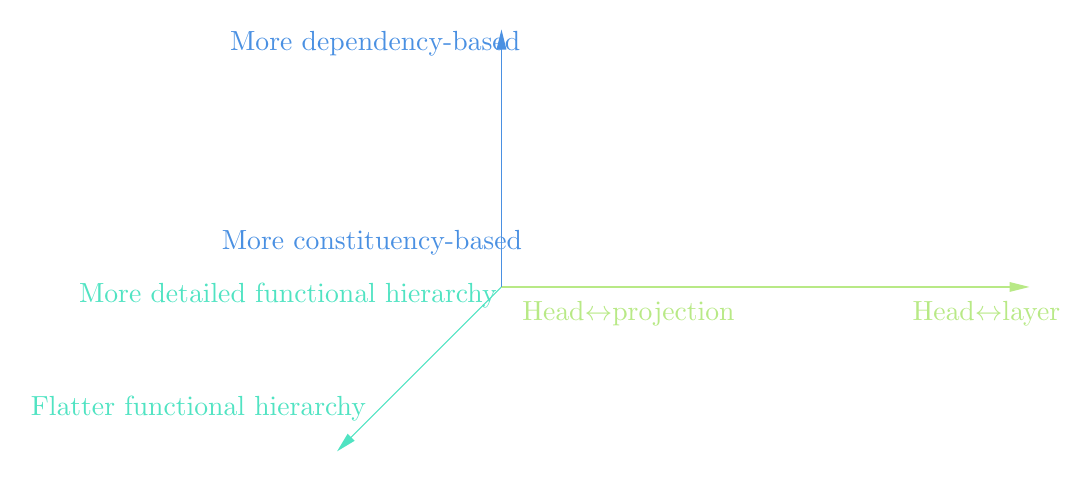
\begin{tikzpicture}[x=0.75pt,y=0.75pt,yscale=-0.8,xscale=0.8]
%uncomment if require: \path (0,536); %set diagram left start at 0, and has height of 536

%Straight Lines [id:da308608375613858] 
\draw [color={rgb, 255:red, 80; green, 227; blue, 194 }  ,draw opacity=1 ]   (323,220.81) -- (225.41,318.4) ;
\draw [shift={(224,319.81)}, rotate = 315] [fill={rgb, 255:red, 80; green, 227; blue, 194 }  ,fill opacity=1 ][line width=0.08]  [draw opacity=0] (12,-3) -- (0,0) -- (12,3) -- cycle    ;
%Straight Lines [id:da6591124487064512] 
\draw [color={rgb, 255:red, 184; green, 233; blue, 134 }  ,draw opacity=1 ]   (323,220.81) -- (639,220.81) ;
\draw [shift={(641,220.81)}, rotate = 180] [fill={rgb, 255:red, 184; green, 233; blue, 134 }  ,fill opacity=1 ][line width=0.08]  [draw opacity=0] (12,-3) -- (0,0) -- (12,3) -- cycle    ;
%Straight Lines [id:da7487030405468103] 
\draw [color={rgb, 255:red, 74; green, 144; blue, 226 }  ,draw opacity=1 ]   (323,220.81) -- (323,67.81) ;
\draw [shift={(323,65.81)}, rotate = 90] [fill={rgb, 255:red, 74; green, 144; blue, 226 }  ,fill opacity=1 ][line width=0.08]  [draw opacity=0] (12,-3) -- (0,0) -- (12,3) -- cycle    ;

% Text Node
\draw (158,65) node [anchor=north west][inner sep=0.75pt]  [color={rgb, 255:red, 74; green, 144; blue, 226 }  ,opacity=1 ] [align=left] {More dependency-based};
% Text Node
\draw (153,185) node [anchor=north west][inner sep=0.75pt]  [color={rgb, 255:red, 74; green, 144; blue, 226 }  ,opacity=1 ] [align=left] {More constituency-based};
% Text Node
\draw (67,217) node [anchor=north west][inner sep=0.75pt]  [color={rgb, 255:red, 80; green, 227; blue, 194 }  ,opacity=1 ] [align=left] {More detailed functional hierarchy};
% Text Node
\draw (38,285) node [anchor=north west][inner sep=0.75pt]  [color={rgb, 255:red, 80; green, 227; blue, 194 }  ,opacity=1 ] [align=left] {Flatter functional hierarchy};
% Text Node
\draw (334,228) node [anchor=north west][inner sep=0.75pt]  [color={rgb, 255:red, 184; green, 233; blue, 134 }  ,opacity=1 ] [align=left] {Head$\displaystyle \leftrightarrow $projection};
% Text Node
\draw (569,228) node [anchor=north west][inner sep=0.75pt]  [color={rgb, 255:red, 184; green, 233; blue, 134 }  ,opacity=1 ] [align=left] {Head$\displaystyle \leftrightarrow $layer};


\end{tikzpicture}

    \caption{Coordinates of equivalent Minimalism formalisms} 
    \label{fig:coordinate-minimalism}
\end{figure}

\prettyref{fig:coordinate-minimalism} gives a coordinate system which classifies possible equivalent formalisms
of Minimalism. \prettyref{fig:minimalism-mapping} illustrates how to explicitly build correspondence between 
different formalisms. In the following sections, I will talk about the three axes in these two figures. 

\begin{figure}
    \centering
    

\tikzset{every picture/.style={line width=0.75pt}} %set default line width to 0.75pt        

\begin{tikzpicture}[x=0.75pt,y=0.75pt,yscale=-0.8,xscale=0.8]
%uncomment if require: \path (0,681); %set diagram left start at 0, and has height of 681

%Straight Lines [id:da8350432578634659] 
\draw [color={rgb, 255:red, 74; green, 144; blue, 226 }  ,draw opacity=1 ]   (255,245) -- (255,186.48) ;
\draw [shift={(255,184.48)}, rotate = 90] [fill={rgb, 255:red, 74; green, 144; blue, 226 }  ,fill opacity=1 ][line width=0.08]  [draw opacity=0] (12,-3) -- (0,0) -- (12,3) -- cycle    ;
%Straight Lines [id:da12751595974157381] 
\draw    (276,319.52) -- (247,333.67) ;
%Straight Lines [id:da4633755411504048] 
\draw    (276,319.52) -- (305,333.67) ;
%Straight Lines [id:da6038585662271874] 
\draw    (305,356.67) -- (334,370.81) ;
%Straight Lines [id:da9621669176728602] 
\draw    (305,356.67) -- (276,370.81) ;
%Straight Lines [id:da22404281311176066] 
\draw    (334,397.81) -- (305,411.96) ;
%Straight Lines [id:da5964038780217018] 
\draw    (334,397.81) -- (363,411.96) ;
%Straight Lines [id:da29518019147428043] 
\draw    (247,281.52) -- (218,295.67) ;
%Straight Lines [id:da8313217199991596] 
\draw    (247,281.52) -- (276,295.67) ;

%Straight Lines [id:da6794750732287518] 
\draw [color={rgb, 255:red, 184; green, 233; blue, 134 }  ,draw opacity=1 ]   (351,322.81) -- (479,322.81) ;
\draw [shift={(481,322.81)}, rotate = 180] [fill={rgb, 255:red, 184; green, 233; blue, 134 }  ,fill opacity=1 ][line width=0.08]  [draw opacity=0] (12,-3) -- (0,0) -- (12,3) -- cycle    ;
%Straight Lines [id:da6367630865324176] 
\draw [color={rgb, 255:red, 80; green, 227; blue, 194 }  ,draw opacity=1 ]   (219,450.33) -- (165.75,503.59) ;
\draw [shift={(164.33,505)}, rotate = 315] [fill={rgb, 255:red, 80; green, 227; blue, 194 }  ,fill opacity=1 ][line width=0.08]  [draw opacity=0] (12,-3) -- (0,0) -- (12,3) -- cycle    ;
%Curve Lines [id:da06681999455732557] 
\draw [color={rgb, 255:red, 0; green, 0; blue, 0 }  ,draw opacity=1 ]   (247,82.48) .. controls (249.97,21.1) and (205.9,17.55) .. (200.16,80.55) ;
\draw [shift={(200,82.48)}, rotate = 274.4] [fill={rgb, 255:red, 0; green, 0; blue, 0 }  ,fill opacity=1 ][line width=0.08]  [draw opacity=0] (12,-3) -- (0,0) -- (12,3) -- cycle    ;
%Curve Lines [id:da9010875284671609] 
\draw [color={rgb, 255:red, 0; green, 0; blue, 0 }  ,draw opacity=1 ]   (252,82.48) .. controls (254.96,21.41) and (289.93,38.93) .. (294.8,81.52) ;
\draw [shift={(295,83.48)}, rotate = 264.81] [fill={rgb, 255:red, 0; green, 0; blue, 0 }  ,fill opacity=1 ][line width=0.08]  [draw opacity=0] (12,-3) -- (0,0) -- (12,3) -- cycle    ;
%Curve Lines [id:da47726983599244965] 
\draw [color={rgb, 255:red, 0; green, 0; blue, 0 }  ,draw opacity=1 ]   (304,81.48) .. controls (311.88,30.26) and (334.31,39.19) .. (338.81,81.52) ;
\draw [shift={(339,83.48)}, rotate = 264.81] [fill={rgb, 255:red, 0; green, 0; blue, 0 }  ,fill opacity=1 ][line width=0.08]  [draw opacity=0] (12,-3) -- (0,0) -- (12,3) -- cycle    ;
%Straight Lines [id:da8683620573651061] 
\draw    (158,574.52) -- (129,588.67) ;
%Straight Lines [id:da9777039126657969] 
\draw    (158,574.52) -- (187,588.67) ;
%Straight Lines [id:da8447403595321143] 
\draw    (583,319.52) -- (554,333.67) ;
%Straight Lines [id:da44472664370190573] 
\draw    (583,319.52) -- (612,333.67) ;
%Straight Lines [id:da546029464490396] 
\draw    (612,356.67) -- (641,370.81) ;
%Straight Lines [id:da25880810260479525] 
\draw    (612,356.67) -- (583,370.81) ;
%Straight Lines [id:da22632049791342013] 
\draw    (641,397.81) -- (612,411.96) ;
%Straight Lines [id:da2708332831470359] 
\draw    (641,397.81) -- (670,411.96) ;
%Straight Lines [id:da565274229303256] 
\draw    (554,281.52) -- (525,295.67) ;
%Straight Lines [id:da22642754581436475] 
\draw    (554,281.52) -- (583,295.67) ;
%Curve Lines [id:da506914942091861] 
\draw    (149,111.15) .. controls (160.94,169.85) and (247.13,184) .. (250.95,110.26) ;
\draw [shift={(251,109.15)}, rotate = 92.29] [fill={rgb, 255:red, 0; green, 0; blue, 0 }  ][line width=0.08]  [draw opacity=0] (12,-3) -- (0,0) -- (12,3) -- cycle    ;
%Straight Lines [id:da7103129253762701] 
\draw [color={rgb, 255:red, 184; green, 233; blue, 134 }  ,draw opacity=1 ]   (367,81.81) -- (468,81.81) ;
\draw [shift={(470,81.81)}, rotate = 180] [fill={rgb, 255:red, 184; green, 233; blue, 134 }  ,fill opacity=1 ][line width=0.08]  [draw opacity=0] (12,-3) -- (0,0) -- (12,3) -- cycle    ;
\draw [shift={(365,81.81)}, rotate = 0] [fill={rgb, 255:red, 184; green, 233; blue, 134 }  ,fill opacity=1 ][line width=0.08]  [draw opacity=0] (12,-3) -- (0,0) -- (12,3) -- cycle    ;
%Curve Lines [id:da597831463173695] 
\draw [color={rgb, 255:red, 0; green, 0; blue, 0 }  ,draw opacity=1 ]   (690,116.15) .. controls (667.12,144.01) and (589.78,173.85) .. (558.47,112.08) ;
\draw [shift={(558,111.15)}, rotate = 63.8] [fill={rgb, 255:red, 0; green, 0; blue, 0 }  ,fill opacity=1 ][line width=0.08]  [draw opacity=0] (12,-3) -- (0,0) -- (12,3) -- cycle    ;
%Curve Lines [id:da9028213106273151] 
\draw [color={rgb, 255:red, 0; green, 0; blue, 0 }  ,draw opacity=1 ]   (694,78.15) .. controls (671.35,24.96) and (652.57,41.62) .. (648.19,81.64) ;
\draw [shift={(648,83.48)}, rotate = 275.53] [fill={rgb, 255:red, 0; green, 0; blue, 0 }  ,fill opacity=1 ][line width=0.08]  [draw opacity=0] (12,-3) -- (0,0) -- (12,3) -- cycle    ;
%Curve Lines [id:da6504393632480485] 
\draw [color={rgb, 255:red, 0; green, 0; blue, 0 }  ,draw opacity=1 ]   (704,77.15) .. controls (711.96,25.41) and (597.16,-29.3) .. (598.96,82.45) ;
\draw [shift={(599,84.15)}, rotate = 268.49] [fill={rgb, 255:red, 0; green, 0; blue, 0 }  ,fill opacity=1 ][line width=0.08]  [draw opacity=0] (12,-3) -- (0,0) -- (12,3) -- cycle    ;
%Curve Lines [id:da09829751807839493] 
\draw    (503.13,114.2) .. controls (541.33,213.66) and (656.45,189.41) .. (701,116.15) ;
\draw [shift={(502,111.15)}, rotate = 70.24] [fill={rgb, 255:red, 0; green, 0; blue, 0 }  ][line width=0.08]  [draw opacity=0] (12,-3) -- (0,0) -- (12,3) -- cycle    ;
%Straight Lines [id:da530044878478577] 
\draw [color={rgb, 255:red, 74; green, 144; blue, 226 }  ,draw opacity=1 ]   (591,256) -- (591,197.48) ;
\draw [shift={(591,195.48)}, rotate = 90] [fill={rgb, 255:red, 74; green, 144; blue, 226 }  ,fill opacity=1 ][line width=0.08]  [draw opacity=0] (12,-3) -- (0,0) -- (12,3) -- cycle    ;
%Straight Lines [id:da17675280085880618] 
\draw    (131,537.52) -- (102,551.67) ;
%Straight Lines [id:da5903649030458693] 
\draw    (131,537.52) -- (160,551.67) ;
%Straight Lines [id:da22079682147404922] 
\draw    (535,574.52) -- (506,588.67) ;
%Straight Lines [id:da9029576654459877] 
\draw    (535,574.52) -- (564,588.67) ;
%Straight Lines [id:da1925387302840138] 
\draw    (508,537.52) -- (479,551.67) ;
%Straight Lines [id:da101307011931842] 
\draw    (508,537.52) -- (537,551.67) ;
%Straight Lines [id:da17160787754640627] 
\draw [color={rgb, 255:red, 184; green, 233; blue, 134 }  ,draw opacity=1 ]   (288,595.81) -- (416,595.81) ;
\draw [shift={(418,595.81)}, rotate = 180] [fill={rgb, 255:red, 184; green, 233; blue, 134 }  ,fill opacity=1 ][line width=0.08]  [draw opacity=0] (12,-3) -- (0,0) -- (12,3) -- cycle    ;
%Straight Lines [id:da8779914022363882] 
\draw [color={rgb, 255:red, 80; green, 227; blue, 194 }  ,draw opacity=1 ]   (622,460.33) -- (568.75,513.59) ;
\draw [shift={(567.33,515)}, rotate = 315] [fill={rgb, 255:red, 80; green, 227; blue, 194 }  ,fill opacity=1 ][line width=0.08]  [draw opacity=0] (12,-3) -- (0,0) -- (12,3) -- cycle    ;
%Straight Lines [id:da3995619192925306] 
\draw [color={rgb, 255:red, 80; green, 227; blue, 194 }  ,draw opacity=1 ]   (130,151.33) -- (76.75,204.59) ;
\draw [shift={(75.33,206)}, rotate = 315] [fill={rgb, 255:red, 80; green, 227; blue, 194 }  ,fill opacity=1 ][line width=0.08]  [draw opacity=0] (12,-3) -- (0,0) -- (12,3) -- cycle    ;
%Straight Lines [id:da989139903952883] 
\draw [color={rgb, 255:red, 74; green, 144; blue, 226 }  ,draw opacity=1 ]   (74,498) -- (74,393.48) ;
\draw [shift={(74,391.48)}, rotate = 90] [fill={rgb, 255:red, 74; green, 144; blue, 226 }  ,fill opacity=1 ][line width=0.08]  [draw opacity=0] (12,-3) -- (0,0) -- (12,3) -- cycle    ;
%Curve Lines [id:da7984911867977953] 
\draw [color={rgb, 255:red, 0; green, 0; blue, 0 }  ,draw opacity=1 ]   (15,300.48) .. controls (14.01,212.59) and (133.79,212.15) .. (126.13,300.15) ;
\draw [shift={(126,301.48)}, rotate = 275.75] [fill={rgb, 255:red, 0; green, 0; blue, 0 }  ,fill opacity=1 ][line width=0.08]  [draw opacity=0] (12,-3) -- (0,0) -- (12,3) -- cycle    ;
%Curve Lines [id:da07667237326010312] 
\draw [color={rgb, 255:red, 0; green, 0; blue, 0 }  ,draw opacity=1 ]   (105,298.48) .. controls (107.97,237.1) and (60.95,237.47) .. (55.16,300.55) ;
\draw [shift={(55,302.48)}, rotate = 274.4] [fill={rgb, 255:red, 0; green, 0; blue, 0 }  ,fill opacity=1 ][line width=0.08]  [draw opacity=0] (12,-3) -- (0,0) -- (12,3) -- cycle    ;

% Text Node
\draw (192,88.55) node [anchor=north west][inner sep=0.75pt]   [align=left] {XP};
% Text Node
\draw (250,88.55) node [anchor=north] [inner sep=0.75pt]  [color={rgb, 255:red, 0; green, 0; blue, 0 }  ,opacity=1 ] [align=left] {F1};
% Text Node
\draw (293,88.55) node [anchor=north] [inner sep=0.75pt]  [color={rgb, 255:red, 0; green, 0; blue, 0 }  ,opacity=1 ] [align=left] {F2};
% Text Node
\draw (339,88.55) node [anchor=north] [inner sep=0.75pt]   [align=left] {√Y};
% Text Node
\draw (220,12) node [anchor=north west][inner sep=0.75pt]  [color={rgb, 255:red, 0; green, 0; blue, 0 }  ,opacity=1 ] [align=left] {1};
% Text Node
\draw (264,20) node [anchor=north west][inner sep=0.75pt]  [color={rgb, 255:red, 0; green, 0; blue, 0 }  ,opacity=1 ] [align=left] {2};
% Text Node
\draw (158,571.52) node [anchor=south] [inner sep=0.75pt]   [align=left] {$>$};
% Text Node
\draw (129,591.67) node [anchor=north] [inner sep=0.75pt]   [align=left] {XP};
% Text Node
\draw (187,591.67) node [anchor=north] [inner sep=0.75pt]   [align=left] {Y$\displaystyle _{\text{[F1, F2]}}$};
% Text Node
\draw (276,316.52) node [anchor=south] [inner sep=0.75pt]   [align=left] {$>$};
% Text Node
\draw (247,336.67) node [anchor=north] [inner sep=0.75pt]   [align=left] {XP};
% Text Node
\draw (305,336.67) node [anchor=north] [inner sep=0.75pt]   [align=left] {$<$};
% Text Node
\draw (276,373.81) node [anchor=north] [inner sep=0.75pt]   [align=left] {F1};
% Text Node
\draw (334,373.81) node [anchor=north] [inner sep=0.75pt]   [align=left] {$<$};
% Text Node
\draw (305,414.96) node [anchor=north] [inner sep=0.75pt]   [align=left] {F2};
% Text Node
\draw (363,414.96) node [anchor=north] [inner sep=0.75pt]   [align=left] {√Y};
% Text Node
\draw (247,278.52) node [anchor=south] [inner sep=0.75pt]   [align=left] {$<$};
% Text Node
\draw (218,298.67) node [anchor=north] [inner sep=0.75pt]   [align=left] {F0};
% Text Node
\draw (583,316.52) node [anchor=south] [inner sep=0.75pt]   [align=left] {$>$};
% Text Node
\draw (554,336.67) node [anchor=north] [inner sep=0.75pt]   [align=left] {XP};
% Text Node
\draw (612,336.67) node [anchor=north] [inner sep=0.75pt]   [align=left] {$>$};
% Text Node
\draw (583,373.81) node [anchor=north] [inner sep=0.75pt]   [align=left] {F1};
% Text Node
\draw (641,373.81) node [anchor=north] [inner sep=0.75pt]   [align=left] {$>$};
% Text Node
\draw (612,414.96) node [anchor=north] [inner sep=0.75pt]   [align=left] {F2};
% Text Node
\draw (670,414.96) node [anchor=north] [inner sep=0.75pt]   [align=left] {√Y};
% Text Node
\draw (554,278.52) node [anchor=south] [inner sep=0.75pt]   [align=left] {$>$};
% Text Node
\draw (525,298.67) node [anchor=north] [inner sep=0.75pt]   [align=left] {F0};
% Text Node
\draw (147,88.48) node [anchor=north] [inner sep=0.75pt]  [color={rgb, 255:red, 0; green, 0; blue, 0 }  ,opacity=1 ] [align=left] {F0};
% Text Node
\draw (545,88.55) node [anchor=north west][inner sep=0.75pt]   [align=left] {XP};
% Text Node
\draw (603,88.55) node [anchor=north] [inner sep=0.75pt]  [color={rgb, 255:red, 0; green, 0; blue, 0 }  ,opacity=1 ] [align=left] {F1};
% Text Node
\draw (646,88.55) node [anchor=north] [inner sep=0.75pt]  [color={rgb, 255:red, 0; green, 0; blue, 0 }  ,opacity=1 ] [align=left] {F2};
% Text Node
\draw (692,88.55) node [anchor=north] [inner sep=0.75pt]   [align=left] {√Y};
% Text Node
\draw (582,160) node [anchor=north west][inner sep=0.75pt]  [color={rgb, 255:red, 0; green, 0; blue, 0 }  ,opacity=1 ] [align=left] {1};
% Text Node
\draw (603,8) node [anchor=north west][inner sep=0.75pt]  [color={rgb, 255:red, 0; green, 0; blue, 0 }  ,opacity=1 ] [align=left] {3};
% Text Node
\draw (500,88.48) node [anchor=north] [inner sep=0.75pt]  [color={rgb, 255:red, 0; green, 0; blue, 0 }  ,opacity=1 ] [align=left] {F0};
% Text Node
\draw (606,128) node [anchor=north west][inner sep=0.75pt]  [color={rgb, 255:red, 0; green, 0; blue, 0 }  ,opacity=1 ] [align=left] {2};
% Text Node
\draw (640,43) node [anchor=north west][inner sep=0.75pt]  [color={rgb, 255:red, 0; green, 0; blue, 0 }  ,opacity=1 ] [align=left] {4};
% Text Node
\draw (370,29) node [anchor=north west][inner sep=0.75pt]  [color={rgb, 255:red, 184; green, 233; blue, 134 }  ,opacity=1 ] [align=left] {moving the end of the arrow \\within the same layer};
% Text Node
\draw (377,341) node [anchor=north west][inner sep=0.75pt]  [color={rgb, 255:red, 184; green, 233; blue, 134 }  ,opacity=1 ] [align=left] {flip $>$ and $<$};
% Text Node
\draw (270,190) node [anchor=north west][inner sep=0.75pt]  [color={rgb, 255:red, 74; green, 144; blue, 226 }  ,opacity=1 ] [align=left] {draw dependency line between \\the head and its dependents};
% Text Node
\draw (312,462.15) node [anchor=north west][inner sep=0.75pt]  [color={rgb, 255:red, 80; green, 227; blue, 194 }  ,opacity=1 ] [align=left] {collapse a functional \\projection span};
% Text Node
\draw (131,534.52) node [anchor=south] [inner sep=0.75pt]   [align=left] {$<$};
% Text Node
\draw (102,554.67) node [anchor=north] [inner sep=0.75pt]   [align=left] {F0};
% Text Node
\draw (535,571.52) node [anchor=south] [inner sep=0.75pt]   [align=left] {$>$};
% Text Node
\draw (506,591.67) node [anchor=north] [inner sep=0.75pt]   [align=left] {XP};
% Text Node
\draw (564,591.67) node [anchor=north] [inner sep=0.75pt]   [align=left] {Y$\displaystyle _{\text{[F1, F2]}}$};
% Text Node
\draw (508,534.52) node [anchor=south] [inner sep=0.75pt]   [align=left] {$>$};
% Text Node
\draw (479,554.67) node [anchor=north] [inner sep=0.75pt]   [align=left] {F0};
% Text Node
\draw (314,571) node [anchor=north west][inner sep=0.75pt]  [color={rgb, 255:red, 184; green, 233; blue, 134 }  ,opacity=1 ] [align=left] {flip $>$ and $<$};
% Text Node
\draw (14,96.15) node [anchor=north west][inner sep=0.75pt]  [color={rgb, 255:red, 80; green, 227; blue, 194 }  ,opacity=1 ] [align=left] {combine several\\dependency \\lines};
% Text Node
\draw (64,315.67) node [anchor=north] [inner sep=0.75pt]   [align=left] {XP};
% Text Node
\draw (122,313.17) node [anchor=north] [inner sep=0.75pt]   [align=left] {Y$\displaystyle _{\text{[F1, F2]}}$};
% Text Node
\draw (16,315.67) node [anchor=north] [inner sep=0.75pt]   [align=left] {F0};


\end{tikzpicture}

    \caption{Mapping between equivalent formalisms}
    \label{fig:minimalism-mapping}
\end{figure}

There is yet a final coordinate of formalisms equivalent to Minimalism: pre-compiled trees 
(read: ``construction''). I will not talk about this topic too much in this section, because there is no 
single way to routinize Minimalism derivations, so routinization cannot be easily represented 
using a coordinate system like \prettyref{fig:coordinate-minimalism}.. 

\subsubsection{Dependency vs constituency}

Dependency relations

\subsubsection{Divergent standards of constituency}

Note that in the above discussion, a word -- a bundle of several features spelt-out together -- is a \emph{span}
and not a constituent in the generative sense, and yet people recognize it as a construction. This % TODO

So now we can see there is no conflict between the binary branching definition of \emph{verb phrase} as Aux plus V plus NP_{\text{object}} and the \ac{blt} definition of verb phrase. A good choice is to use the term 
\emph{verb complex} to denote verb phrase in the \ac{blt} sense \citep{Wilbur2014}.

There is yet a final issue about how flat the syntax tree should be. It is kind of strange to talk about 
flat trees in a theory equivalent to Minimalism, but recall that in lexicalist Minimalism, a terminal node 
in a syntactic tree can have unrestrictedly large feature bundles i.e. unrestricted branching, and 
we know lexicalist Minimalism can be seen as an equivalent formalism of OFOH Minimalism, it is nature 
to ask whether unrestricted branching for \emph{all} kinds of nodes -- not just feature nodes -- also gives 
an equivalent grammar class to the grammar class allowed in Minimalism.

Take the tree structure of a simple clause as an example. In \ac{blt}, Dixon accuses the binary division between 
the subject and the predicate as harmful (without providing much argumentation about it), but when discussing 
topic and pivots, he distinguishes the subject (in accusative languages, of course) from other arguments and regards it as having a somehow more 
prominent position. The arguments are licensed by the verb and have dependency relations with the verb. 
Introducing a position of pivot (or subject in accusative languages) besides the notion of deep S, A and O 
of course means introducing a layer of construction built \emph{upon} the argument structure layer
about ``the obligatory and syntactically codified topic'', 
which, in generative terms, is just the TP layer. It is of course possible to draw a syntactic tree 
with a quite flat clause structure and explain that ``the subject somehow has a higher position'', 
but this is eventually the same as the binary branch approach in Minimalism.

\begin{figure}
    \centering
    

\tikzset{every picture/.style={line width=0.75pt}} %set default line width to 0.75pt        

\begin{tikzpicture}[x=0.75pt,y=0.75pt,yscale=-1,xscale=1]
%uncomment if require: \path (0,577); %set diagram left start at 0, and has height of 577

%Straight Lines [id:da3571919269318433] 
\draw    (294,104.56) -- (265,118.71) ;
%Straight Lines [id:da6561258080060619] 
\draw    (294,104.56) -- (323,118.71) ;
%Straight Lines [id:da06898664551834899] 
\draw    (321,147.48) -- (358,165.85) ;
%Straight Lines [id:da8075756397517635] 
\draw    (321,147.48) -- (285,164.48) ;
%Straight Lines [id:da41665955900317875] 
\draw    (358,192.85) -- (329,207) ;
%Straight Lines [id:da9079604504645364] 
\draw    (358,192.85) -- (387,207) ;
%Straight Lines [id:da7478179026703973] 
\draw    (239,54.48) -- (187,78.71) ;
%Straight Lines [id:da456511156570109] 
\draw    (239,54.48) -- (290,78.71) ;
%Straight Lines [id:da5715409936346081] 
\draw    (386,238.71) -- (415,252.85) ;
%Straight Lines [id:da9144092856943298] 
\draw    (386,238.71) -- (357,252.85) ;
%Straight Lines [id:da550303334673411] 
\draw    (415,276.85) -- (386,291) ;
%Straight Lines [id:da5505916969954645] 
\draw    (415,276.85) -- (444,291) ;
%Straight Lines [id:da848474007635855] 
\draw    (443,322.71) -- (472,336.85) ;
%Straight Lines [id:da4690731977225433] 
\draw    (443,322.71) -- (414,336.85) ;
%Shape: Ellipse [id:dp6349484937583538] 
\draw   (241,110.35) .. controls (251.36,101.76) and (275.54,113.86) .. (294.99,137.36) .. controls (314.45,160.86) and (321.82,186.87) .. (311.45,195.45) .. controls (301.08,204.03) and (276.91,191.94) .. (257.45,168.44) .. controls (237.99,144.94) and (230.63,118.93) .. (241,110.35) -- cycle ;
%Curve Lines [id:da13670515659331373] 
\draw [color={rgb, 255:red, 155; green, 155; blue, 155 }  ,draw opacity=1 ]   (254,163.48) .. controls (208.46,148.63) and (205.06,160.24) .. (182.68,201.73) ;
\draw [shift={(182,203)}, rotate = 298.41] [fill={rgb, 255:red, 155; green, 155; blue, 155 }  ,fill opacity=1 ][line width=0.08]  [draw opacity=0] (12,-3) -- (0,0) -- (12,3) -- cycle    ;
%Shape: Ellipse [id:dp6152794315221408] 
\draw   (318.95,190.86) .. controls (347.52,155.06) and (423.21,167.96) .. (488.01,219.67) .. controls (552.81,271.38) and (582.18,342.33) .. (553.61,378.13) .. controls (525.04,413.93) and (449.35,401.03) .. (384.55,349.32) .. controls (319.75,297.61) and (290.38,226.67) .. (318.95,190.86) -- cycle ;
%Curve Lines [id:da73255009866522] 
\draw  [dash pattern={on 4.5pt off 4.5pt}]  (337.8,269.11) .. controls (299.4,323.15) and (369.03,405.1) .. (471,367.48) ;
\draw [shift={(339,267.48)}, rotate = 127.21] [fill={rgb, 255:red, 0; green, 0; blue, 0 }  ][line width=0.08]  [draw opacity=0] (12,-3) -- (0,0) -- (12,3) -- cycle    ;
%Curve Lines [id:da5371088007693434] 
\draw  [dash pattern={on 4.5pt off 4.5pt}]  (345.87,273.79) .. controls (342.98,323.87) and (342.8,336.72) .. (395,352.48) ;
\draw [shift={(346,271.48)}, rotate = 93.3] [fill={rgb, 255:red, 0; green, 0; blue, 0 }  ][line width=0.08]  [draw opacity=0] (12,-3) -- (0,0) -- (12,3) -- cycle    ;
%Shape: Ellipse [id:dp4170769301823447] 
\draw   (329,237.35) .. controls (339.36,228.76) and (356.94,232.88) .. (368.25,246.54) .. controls (379.56,260.21) and (380.33,278.24) .. (369.96,286.83) .. controls (359.59,295.41) and (342.02,291.29) .. (330.7,277.63) .. controls (319.39,263.96) and (318.63,245.93) .. (329,237.35) -- cycle ;
%Curve Lines [id:da8605216809412348] 
\draw [color={rgb, 255:red, 155; green, 155; blue, 155 }  ,draw opacity=1 ]   (324,266.48) .. controls (270.54,268.46) and (265.1,275.34) .. (210.66,259.95) ;
\draw [shift={(209,259.48)}, rotate = 15.95] [fill={rgb, 255:red, 155; green, 155; blue, 155 }  ,fill opacity=1 ][line width=0.08]  [draw opacity=0] (12,-3) -- (0,0) -- (12,3) -- cycle    ;
%Shape: Ellipse [id:dp9342228745072949] 
\draw   (133.13,175.12) .. controls (149.65,161.45) and (184.75,176.58) .. (211.52,208.92) .. controls (238.3,241.26) and (246.61,278.57) .. (230.09,292.24) .. controls (213.57,305.92) and (178.47,290.79) .. (151.7,258.44) .. controls (124.93,226.1) and (116.61,188.8) .. (133.13,175.12) -- cycle ;
%Curve Lines [id:da026296240479518618] 
\draw    (321,218.48) .. controls (214.08,221.45) and (186.55,154.83) .. (186.98,108.87) ;
\draw [shift={(187,107.48)}, rotate = 91.25] [fill={rgb, 255:red, 0; green, 0; blue, 0 }  ][line width=0.08]  [draw opacity=0] (12,-3) -- (0,0) -- (12,3) -- cycle    ;
%Shape: Ellipse [id:dp018559860692994645] 
\draw   (49,62.17) .. controls (126.16,-27.48) and (302.23,-2.43) .. (442.27,118.1) .. controls (582.31,238.64) and (633.28,409.02) .. (556.12,498.67) .. controls (478.96,588.31) and (302.89,563.27) .. (162.85,442.73) .. controls (22.81,322.19) and (-28.16,151.81) .. (49,62.17) -- cycle ;

% Text Node
\draw (294,101.56) node [anchor=south] [inner sep=0.75pt]   [align=left] {T'};
% Text Node
\draw (265,121.71) node [anchor=north] [inner sep=0.75pt]   [align=left] {Pres};
% Text Node
\draw (321,125.71) node [anchor=north] [inner sep=0.75pt]   [align=left] {AspP};
% Text Node
\draw (285,167.48) node [anchor=north] [inner sep=0.75pt]   [align=left] {Perf};
% Text Node
\draw (358,168.85) node [anchor=north] [inner sep=0.75pt]   [align=left] {$\displaystyle v$P};
% Text Node
\draw (329,210) node [anchor=north] [inner sep=0.75pt]   [align=left] {\st{I}};
% Text Node
\draw (387,210) node [anchor=north] [inner sep=0.75pt]   [align=left] {$\displaystyle v_{\text{Do}} '$};
% Text Node
\draw (239,51.48) node [anchor=south] [inner sep=0.75pt]   [align=left] {TP};
% Text Node
\draw (357,255.85) node [anchor=north] [inner sep=0.75pt]   [align=left] {Do};
% Text Node
\draw (415,255.85) node [anchor=north] [inner sep=0.75pt]   [align=left] {TransP};
% Text Node
\draw (386,294) node [anchor=north] [inner sep=0.75pt]   [align=left] {[the task]};
% Text Node
\draw (444,294) node [anchor=north] [inner sep=0.75pt]   [align=left] {Trans'};
% Text Node
\draw (414,339.85) node [anchor=north] [inner sep=0.75pt]   [align=left] {Trans};
% Text Node
\draw (187,81.71) node [anchor=north] [inner sep=0.75pt]   [align=left] {I};
% Text Node
\draw (450,339) node [anchor=north west][inner sep=0.75pt]   [align=left] {√COMPLETE};
% Text Node
\draw (468,237) node [anchor=north west][inner sep=0.75pt]   [align=left] {layer 1: \\deep \\argument \\structure};
% Text Node
\draw (165,205) node [anchor=north west][inner sep=0.75pt]   [align=left] {have};
% Text Node
\draw (153,240) node [anchor=north west][inner sep=0.75pt]   [align=left] {completed};
% Text Node
\draw (49,232) node [anchor=north west][inner sep=0.75pt]   [align=left] {verb phrase};
% Text Node
\draw (115,77) node [anchor=north west][inner sep=0.75pt]   [align=left] {layer 3:\\subject\\movement};
% Text Node
\draw (309,431) node [anchor=north west][inner sep=0.75pt]   [align=left] {layer 2:\\basic\\clause \\structure};


\end{tikzpicture}

    \caption{The derivation of \emph{I have completed my task} in Minimalism}
    \label{fig:complete-my-task-minimalism}
\end{figure}

Consider, for example, the derivational process shown in \prettyref{fig:complete-my-task-minimalism}.
This seems complicated because we are only allowed to use Merge and spellout, but we can certainly 
find three routinized processes: the first is to assemble the $v$P structure and to build the argument 
structure, the second is to add tense and aspect information and to spell out them as auxiliary verbs
(hence forming the ``verb phrase'' in the \ac{blt} sense), and the third is the A-movement of the subject.
If we work with these routines instead of Merge and spellout, what we get is exactly the \ac{blt} version 
of tree diagram shown in \prettyref{fig:complete-my-task-blt-1}.

\begin{figure}
    \centering
    

\tikzset{every picture/.style={line width=0.75pt}} %set default line width to 0.75pt        

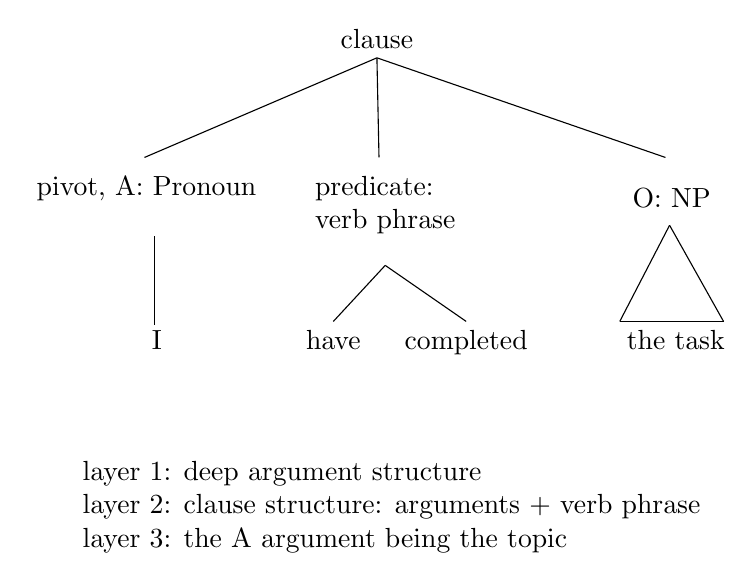
\begin{tikzpicture}[x=0.75pt,y=0.75pt,yscale=-1,xscale=1]
%uncomment if require: \path (0,390); %set diagram left start at 0, and has height of 390

%Straight Lines [id:da4161051988460063] 
\draw    (183,100.81) -- (71,148.81) ;
%Straight Lines [id:da36248311433047187] 
\draw    (187,200.81) -- (162,227.81) ;
%Straight Lines [id:da4439661314753782] 
\draw    (187,200.81) -- (226,227.81) ;
%Straight Lines [id:da36890954567869483] 
\draw    (300,227.81) -- (350,227.81) ;
%Straight Lines [id:da011342458373226894] 
\draw    (324,181.48) -- (300,227.81) ;
%Straight Lines [id:da5435200709744346] 
\draw    (324,181.48) -- (350,227.81) ;
%Straight Lines [id:da24568188379824396] 
\draw    (76,186.81) -- (76,229.48) ;
%Straight Lines [id:da3308532295080375] 
\draw    (183,100.81) -- (184,148.81) ;
%Straight Lines [id:da7487945318074942] 
\draw    (183,100.81) -- (322,148.81) ;

% Text Node
\draw (77,230.81) node [anchor=north] [inner sep=0.75pt]   [align=left] {I};
% Text Node
\draw (162,230.81) node [anchor=north] [inner sep=0.75pt]   [align=left] {have};
% Text Node
\draw (226,230.81) node [anchor=north] [inner sep=0.75pt]   [align=left] {completed};
% Text Node
\draw (327,230.81) node [anchor=north] [inner sep=0.75pt]   [align=left] {the task};
% Text Node
\draw (187,187) node [anchor=south] [inner sep=0.75pt]   [align=left] {predicate:\\verb phrase};
% Text Node
\draw (325,174) node [anchor=south] [inner sep=0.75pt]   [align=left] {O: NP};
% Text Node
\draw (15,157) node [anchor=north west][inner sep=0.75pt]   [align=left] {\begin{minipage}[lt]{83.56pt}\setlength\topsep{0pt}
\begin{center}
pivot, A: Pronoun
\end{center}

\end{minipage}};
% Text Node
\draw (183,97.81) node [anchor=south] [inner sep=0.75pt]   [align=left] {clause};
% Text Node
\draw (40,294) node [anchor=north west][inner sep=0.75pt]   [align=left] {layer 1: deep argument structure\\layer 2: clause structure: arguments + verb phrase\\layer 3: the A argument being the topic};


\end{tikzpicture}

    \caption{The tree diagram representation of \emph{I have completed my task} in \ac{blt}}
    \label{fig:complete-my-task-blt-1}
\end{figure}

We see that every syntactic relation in the \ac{blt} tree diagram traces back to a dependency relation created 
by Merge. The notion of a ``verb phrase'' in the \ac{blt} sense which includes both the verb and the auxiliary 
verb (but not the arguments) is a \emph{span} in generative terms. The deep argument structure is realized 
in the $v$P layer in the Minimalism derivation. The clause structure is the TP layer, and the fact that 
in active clauses the A argument is the pivot is realized by the Spec-$v$P to Spec-TP A-movement.%
\footnote{One question here might be that layer 2 seems to be the T' projection, while layer 3 seems to be 
the SpecTP position and EPP feature, but it seems strange that a construction routinizes an intermediate
projection. But for the sake of conciseness, \prettyref{fig:complete-my-task-minimalism} is \emph{not} 
a true cartographic syntactic tree, and just as the case in \ac{cgel} that a projection corresponding to 
N' in the classical X-bar theory is actually a maximal projection, so is T' in \prettyref{fig:complete-my-task-minimalism}.}
Rejection of fine-grained constituent structure means coexistence of flat trees and dependency relations.
Note that \prettyref{fig:complete-my-task-blt-1} is also a demonstration of a grammar working with 
routinized pre-compiled constructions, not Merge and a list of syntactic atoms. I will 
talk about this in \prettyref{sec:routine}.

A similar case where the loss of structural information in less fine-grained formalisms
is remended by adding additional dependency relations can be found in \ac{cgel} 5.14.1, where 
we have \emph{indirect} complements, which are licensed by another dependent in a phrase, 
and the dependency relation between an indirect complement and its licensor is not that 
transparent in \ac{cgel}'s phrase structure grammar.

\subsubsection{The notion of \emph{head}}\label{sec:headedness}

What is the head of a phrase is also a topic causing lots of disputation. 

So here we see the root cause of the disagreement between Minimalism and the \ac{blt}- or \ac{cgel}-definition 
of head. The former is about labeling a newly introduced element (i.e. the specifier), while the latter is about 
the the overall syntactic function of the whole phrase. 

\subsection{Deriving more surface-oriented formalisms}

\subsubsection{Minimalism as constructivism}\label{sec:routine}

One reason to use pre-compiled trees is derivational theories are sometimes 
practically hard to use when doing computational researches. For example, \citet{liter2020modeling}
is about how fine-grained feature hierarchy simplifies learning, but it has to explicitly solve out what 
a derivational grammatical constraint allows, and then work with the not-so-derivational possibilities.

Another reason to keep pre-compiled trees is it makes the theory more psychologically plausible --
attempts trying to localize Merge in the brain are generally not that successful, and assuming that 
human brains do store constructions, while on the other hand these constructions are still analyzable 
in terms of Merge seems a plausible answer to what is really going on in our brains
\citep{brain-syntax-1,brain-syntax-2}. There are also acquisitional evidences supporting the claim 
that we learn words one by one and not in terms of abstract features \citep{white2022lexicalization},
but abstract features are useful anyway as one method to narrow down possible languages \citep{liter2020modeling}.

A large type of grammars with pre-compiled trees is the type of \concept{lexicalist} grammars, where 
a word is actually a pre-compiled tree, with placeholders in its complement positions, and words 
are the \emph{only} kind of structure-building primitives. % TODO: 两种lexicalist的区别

\subsubsection{Categories and the notion of ``word''}

A \concept{category}\index{category} is defined as a type of constructions with similar distributions.
I will first discuss basic syntactic constructions and identify positions that can be filled in them, 
and then search possible constructions in these positions. This is how categories can be recognized.

A construction that is small enough is said to be a \concept{word} or more precisely, 
a \concept{grammatical word}\index{word!grammatical}.
I emphasize \emph{grammatical} because it is quite common to use the term \emph{word} 词 to denote 
a \concept{prosody word}\index{word!prosody}. Prosody is important in Chinese, which is discussed in 
\prettyref{sec:prosody-intro} and \prettyref{chap:prosody-overview}. 

In traditional grammars concerning Latin, a common practice is to roughly define word classes (nouns, verbs, etc.) 
according to their meaning and then discuss where they can be used. 
In this proto-book I do not take this approach. Though I will review a lot of work based on the meaning-first 
approach, the way I distinguish word classes is mainly distributional. If two words can appear in similar
positions, they are classified into one \concept{word class}\index{word class} or \concept{part of speech}.
A word class is just a category about words.  

In other words, I define concepts like \emph{noun-like} and \emph{verb-like} \emph{before} listing criteria of 
what is a noun and what is a verb. Criteria for word classes are always language-specific, but we have more 
confidence that at least some \emph{features} -- like the nominal feature \textit{n} or the verbal feature 
\textit{v} -- are cross-linguistic and may be attributed to the language faculty in the broad sense. 

\subsubsection{Phrase labels}\label{sec:phrase-label}

% TODO: phrase label作为给出dependency relation的一种方式
% TODO: 扔掉Cinque hierarchy中无用的functional head

The \ac{cgel} approach of dependent types effectively gives us something like the good old X-bar theory, where a lexical word 
(not a functional word, especially not an invisible functional head) heads a phrase with multiple 
complements, specifiers and adjuncts (all in generative terms). The main differences between the GB-like 
X-bar scheme and the \ac{cgel} scheme are that in the former terms like ``complement'' is defined strictly 
in structural terms (e.g. ``the sister of the head''), while in the latter these terms are defined in 
terms of dependency relations (e.g. ``complements are more explicitly licensed by the head than 
modifiers'') without any guarantee that complements are necessarily lower than modifiers \citep{payne2007fusion},
and that in the \ac{cgel} framework there is no intermediate projections: nominals in \ac{cgel} corresponds 
to N' projections in X-bar theory, but the former can appear as a complete unit (e.g. as the modifier of another 
NP). 

We can summarize that the framework in \ac{cgel} is a little more flexible than X-bar theory. 
From the Minimalism perspective, it is easy to explain why: the criteria \ac{cgel} uses to draw the line 
between complements and modifiers are related more to spellout (see the discussion in \prettyref{sec:sub-cat})
than the tree structure and hints nothing about whether a constituent is a maximal projection or not. 
Purely tree structure-based notion of ``complements'' is bond to fail. 
So-called intermediate projections in X-bar theory, like N', are actually maximal projections according to 
more fine-grained analysis, and hence they indeed can appear as a complete phrase.
The X-bar theory is therefore just a transitional version of generative syntax.

\subsubsection{Dependency relations as in dependency grammars}\label{sec:dependency}

\subsubsection{Selection and subcagegorization, complements and modifiers}\label{sec:sub-cat}

It should be noted that the distinction between complements and modifiers are still opaque even with 
all these discussions about licensing and selection, and this opaqueness is theoretically rooted. 
Languages that have a relatively fixed word order often impose (though usually in a rather subtle way) 
a word order constraints on different types of clausal adjuncts and adjectives in NPs, 
which is well explained by the cartographic approach as we see above that the adjuncts and NP modifiers 
are actually introduced by a fixed hierarchy of functional heads. Since we consider the functional heads 
to be realized \emph{onto} the \ac{cgel} head of the construction -- the main noun, the main verb, etc. -- 
it follows that adjectives about different properties fill different ``slots of modifiers'' of the head noun, 
and similarly adjuncts about different properties fill different ``slots of modifiers'' of the head verb, 
in exactly the same way arguments fill argument slots. 

A clear distinction between complements and modifiers -- or in the cause of clause structure, arguments and
adjuncts -- is therefore of limited purely formal interest and is better viewed as a language-specific concept, 
which may be useful for description \citep{haspelmath2014arguments}. 

It should also be noted that the term \emph{argument} is not the same as the term \concept{complement}, 
although the term \emph{argument-adjunct distinction} is much more frequent than the \ac{cgel}-style 
\emph{complement-modifier distinction}.
In \ac{blt}'s terms, an argument % TODO: what's an argument?

Complement clauses are less nominal since across languages they usually do not have person, number, gender and 
case (or so-called \concept{$\phi$-features} in generative terms), but it is still kind of nominal, 
and the complementizer is argued by some people to implicitly carry $\phi$-features \citep{complement-clause}.

\begin{figure}
    \centering
    

\tikzset{every picture/.style={line width=0.75pt}} %set default line width to 0.75pt        

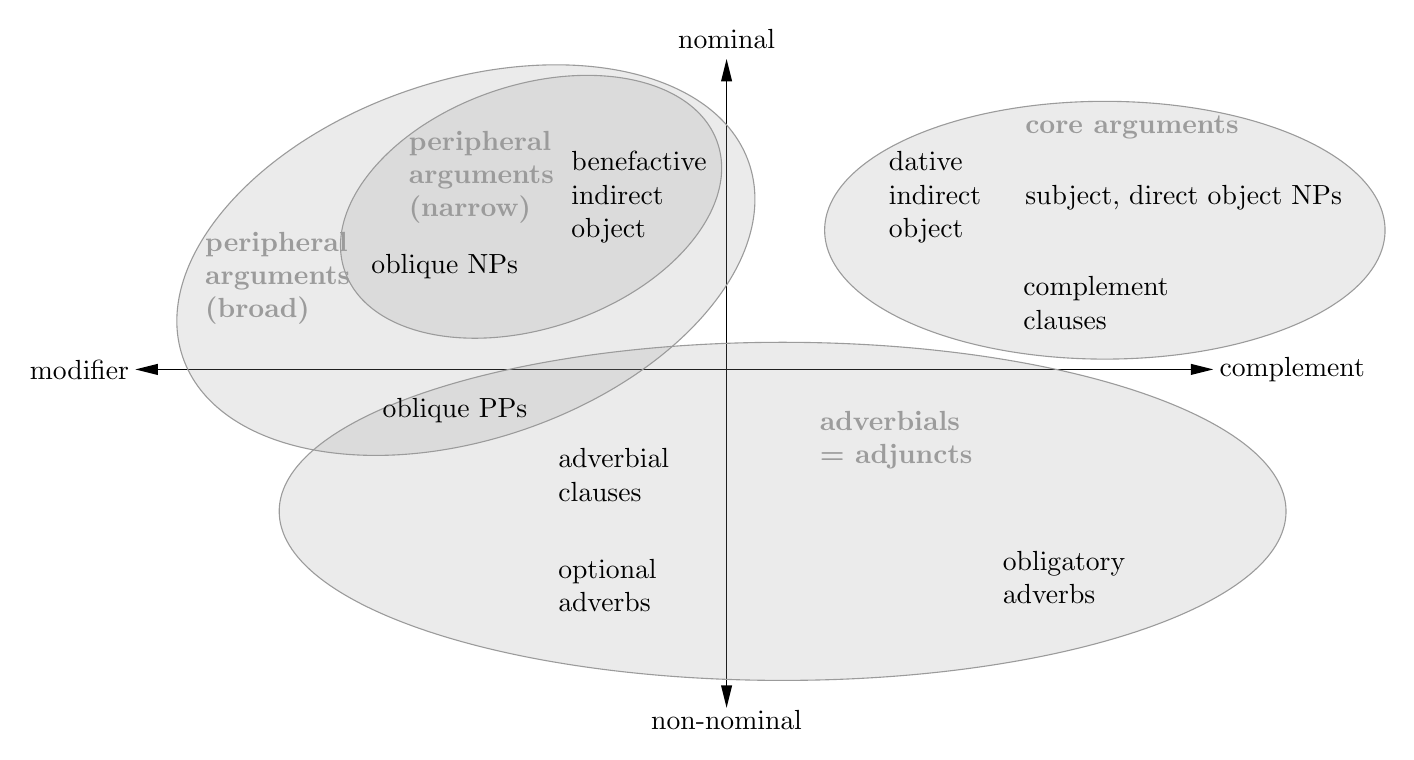
\begin{tikzpicture}[x=0.75pt,y=0.75pt,yscale=-0.9,xscale=0.9]
%uncomment if require: \path (0,401); %set diagram left start at 0, and has height of 401

%Straight Lines [id:da009476237276789146] 
\draw    (98,198) -- (671,198) ;
\draw [shift={(673,198)}, rotate = 180] [fill={rgb, 255:red, 0; green, 0; blue, 0 }  ][line width=0.08]  [draw opacity=0] (12,-3) -- (0,0) -- (12,3) -- cycle    ;
\draw [shift={(96,198)}, rotate = 0] [fill={rgb, 255:red, 0; green, 0; blue, 0 }  ][line width=0.08]  [draw opacity=0] (12,-3) -- (0,0) -- (12,3) -- cycle    ;
%Straight Lines [id:da7773022804601077] 
\draw    (412.5,377.14) -- (412.5,33.86) ;
\draw [shift={(412.5,31.86)}, rotate = 90] [fill={rgb, 255:red, 0; green, 0; blue, 0 }  ][line width=0.08]  [draw opacity=0] (12,-3) -- (0,0) -- (12,3) -- cycle    ;
\draw [shift={(412.5,379.14)}, rotate = 270] [fill={rgb, 255:red, 0; green, 0; blue, 0 }  ][line width=0.08]  [draw opacity=0] (12,-3) -- (0,0) -- (12,3) -- cycle    ;
%Shape: Ellipse [id:dp6612766652403343] 
\draw  [color={rgb, 255:red, 155; green, 155; blue, 155 }  ,draw opacity=1 ][fill={rgb, 255:red, 155; green, 155; blue, 155 }  ,fill opacity=0.2 ] (465,123.48) .. controls (465,85.37) and (532.16,54.48) .. (615,54.48) .. controls (697.84,54.48) and (765,85.37) .. (765,123.48) .. controls (765,161.59) and (697.84,192.48) .. (615,192.48) .. controls (532.16,192.48) and (465,161.59) .. (465,123.48) -- cycle ;
%Shape: Ellipse [id:dp35746311023681887] 
\draw  [color={rgb, 255:red, 155; green, 155; blue, 155 }  ,draw opacity=1 ][fill={rgb, 255:red, 155; green, 155; blue, 155 }  ,fill opacity=0.2 ] (208.04,145.17) .. controls (196.4,111.22) and (231.65,68.38) .. (286.77,49.48) .. controls (341.89,30.57) and (396.01,42.76) .. (407.65,76.71) .. controls (419.29,110.65) and (384.04,153.49) .. (328.92,172.4) .. controls (273.8,191.3) and (219.68,179.11) .. (208.04,145.17) -- cycle ;
%Shape: Ellipse [id:dp7325522804450764] 
\draw  [color={rgb, 255:red, 155; green, 155; blue, 155 }  ,draw opacity=1 ][fill={rgb, 255:red, 155; green, 155; blue, 155 }  ,fill opacity=0.2 ] (121.39,191.46) .. controls (104.22,141.37) and (158.14,77.5) .. (241.84,48.79) .. controls (325.54,20.09) and (407.32,37.42) .. (424.49,87.51) .. controls (441.67,137.6) and (387.75,201.47) .. (304.05,230.18) .. controls (220.35,258.88) and (138.57,241.55) .. (121.39,191.46) -- cycle ;
%Shape: Ellipse [id:dp17093026002033596] 
\draw  [color={rgb, 255:red, 155; green, 155; blue, 155 }  ,draw opacity=1 ][fill={rgb, 255:red, 155; green, 155; blue, 155 }  ,fill opacity=0.2 ] (173,273.98) .. controls (173,224) and (293.66,183.48) .. (442.5,183.48) .. controls (591.34,183.48) and (712,224) .. (712,273.98) .. controls (712,323.96) and (591.34,364.48) .. (442.5,364.48) .. controls (293.66,364.48) and (173,323.96) .. (173,273.98) -- cycle ;

% Text Node
\draw (571,98) node [anchor=north west][inner sep=0.75pt]   [align=left] {subject, direct object NPs};
% Text Node
\draw (675,198) node [anchor=west] [inner sep=0.75pt]   [align=left] {complement};
% Text Node
\draw (94,198) node [anchor=east] [inner sep=0.75pt]   [align=left] {modifier};
% Text Node
\draw (412.5,27.86) node [anchor=south] [inner sep=0.75pt]   [align=left] {nominal};
% Text Node
\draw (412.5,379.14) node [anchor=north] [inner sep=0.75pt]   [align=left] {non-nominal};
% Text Node
\draw (498,80) node [anchor=north west][inner sep=0.75pt]   [align=left] {dative \\indirect \\object};
% Text Node
\draw (570,147) node [anchor=north west][inner sep=0.75pt]   [align=left] {complement \\clauses};
% Text Node
\draw (328,80) node [anchor=north west][inner sep=0.75pt]   [align=left] {benefactive \\indirect \\object};
% Text Node
\draw (221,135) node [anchor=north west][inner sep=0.75pt]   [align=left] {oblique NPs};
% Text Node
\draw (227,212) node [anchor=north west][inner sep=0.75pt]   [align=left] {oblique PPs};
% Text Node
\draw (559,294) node [anchor=north west][inner sep=0.75pt]   [align=left] {obligatory\\adverbs};
% Text Node
\draw (321,298) node [anchor=north west][inner sep=0.75pt]   [align=left] {optional\\adverbs};
% Text Node
\draw (321,239) node [anchor=north west][inner sep=0.75pt]   [align=left] {adverbial \\clauses};
% Text Node
\draw (571,61) node [anchor=north west][inner sep=0.75pt]  [color={rgb, 255:red, 155; green, 155; blue, 155 }  ,opacity=1 ] [align=left] {\textbf{\textcolor[rgb]{0.61,0.61,0.61}{core arguments}}};
% Text Node
\draw (241,69) node [anchor=north west][inner sep=0.75pt]  [color={rgb, 255:red, 155; green, 155; blue, 155 }  ,opacity=1 ] [align=left] {\textbf{peripheral}\\\textbf{arguments}\\\textbf{(narrow)}};
% Text Node
\draw (132,123) node [anchor=north west][inner sep=0.75pt]  [color={rgb, 255:red, 155; green, 155; blue, 155 }  ,opacity=1 ] [align=left] {\textbf{peripheral }\\\textbf{arguments}\\\textbf{(broad)}};
% Text Node
\draw (461,219) node [anchor=north west][inner sep=0.75pt]   [align=left] {\textcolor[rgb]{0.61,0.61,0.61}{\textbf{adverbials}}\\\textbf{\textcolor[rgb]{0.61,0.61,0.61}{= adjuncts}}};


\end{tikzpicture}

    \caption{Classification of clause dependents in typical European languages}
\end{figure}

% TODO: Adjunction, typical structure is described first, then adjunction of optional elements

\subsubsection{Movements}

Whenever dependency relations that cannot be transparently reflected by a phrase structure grammar occur,
movements occur.

\subsubsection{Empty categories and fusion-function constructions}

\subsubsection{Feature structures}


\section{Descriptive terms}

I have paid length discussions of \emph{structures} and demonstrated that the superfluously diverging 
frameworks are actually almost the same. But the formalism of generative syntax is probably not 
what dissatisfies field linguists the most.
Having worked out a \emph{formal} grammatical framework, a list of \emph{building blocks} 
are still required for fully describing a language. The former is purely about 
how structures are built, while the latter is about what raw materials are fed into the structure 
building machine. Universals about the former and the latter are called formal and substantial universals,
respectively. Now readers of \ac{blt} will find what Dixon complains most about is not about the 
binary branching trees, but the tendency of ``formalists'' to find things equivalent to English 
in newly documented languages. In his depiction, formalists assume there are infinitives, 
inflection-derivation distinction, etc. in all languages, which he mocks several times. 
This depiction is actually not quite true for most generative works but is 
alarming for people seeking language universals % TODO

\subsection{Clause structure}

We use the term \concept{verb phrase (VP)} to denote % TODO: if there is V to T movement?
% Predicator,NP等概念 argument structure 见syntax within the word一书

% BLT, CGEL, 中比较实质性的概念

\subsection{Noun phrases}

The term \concept{nominal}\index{nominal} is used mostly as an adjective. Since Chinese does not have 
explicitly the determiner position, we do not need a separate term for NP-like phrases without a determiner.
So, despite the fact \ac{cgel} uses the term \emph{nominal} to denote constituents like \emph{red apple}, 
this proto-book uses the term \emph{nominal} to denote anything that is noun-like.

\section{Data sources}

% 关于语料来源和分析方法

\end{document}